\chapter{Uso de Licenças Creative Commons}
As licenças Creative Commons são uma família de licenças copyleft criada e
mantida pela organização não comercial Creative Commons. Atualmente as licenças
Creative Commons Atribuição 3.0 Não Adaptada (CC-BY) e Creative Commons
Atribuição-CompartilhaIgual 3.0 Não Adaptada (CC-BY-SA) são as licenças mais
utilizadas em conteúdos/recursos abertos.

Os mantenedores deste modelo sugerem a utilizado das licenças CC-BY e CC-BY-SA
por acreditarem que a ciência é melhor desenvolvida quando:
\begin{itemize}
  \item pesquisadores possam compartilhar, utilizar e remixar o trabalho de seus
    colegas (sob a condição de dar os devidos créditos) e
  \item não tenham que se preocupar com a violação de direitos autorais (desde
    que faça atribuição ao autor e trabalho original).
\end{itemize}
Essas são as características de materiais licenciados utilizando CC-BY ou
CC-BY-SA e por isso incentivamos seu uso.

Nas próximas seções você encontrará maiores detalhes sobre as licenças CC-BY e
CC-BY-SA, como utilizá-las em sua dissertação de mestrado ou tese de doutorado e
informações adicionais.

\section{Creative Commons Atribuição 3.0 Não Adaptada}
A licença Creative Commons Atribuição 3.0 Não Adaptada (CC-BY) é a menos restritiva das
licenças Creative Commons. Um material que utiliza essa licença pode ser:
\begin{itemize}
  \item copiado,
  \item distribuído e
  \item modificado
\end{itemize}
por qualquer pessoa desde que indique a obra original e seu autor. Para maiores
informações visite
\url{http://creativecommons.org/licenses/by/3.0/deed.pt_BR}.


Para utilizá-la na sua dissertação de mestrado ou tese de doutorado,
certifique-se do arquivo \lstinline+cc-by.tex+ ter sido incluso no arquivo
\lstinline+tese.tex+ como indicado abaixo:
\begin{lstlisting}
\annex
% TODO Inserir os arquivos referentes aos apendices e anexos.
\chapter{Licença}
Copyright (c) \ano \ de \autor.

Exceto quando indicado o contrário, esta obra está licenciada sob a licença
Creative Commons Atribuição 3.0 Não Adaptada. Para ver uma cópia desta licença,
visite \url{http://creativecommons.org/licenses/by/3.0/}.

\begin{center}
  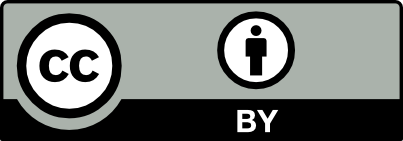
\includegraphics{figuras/cc-by.png}
\end{center}

%%%%%%%%%%%%%%%%%%%%%%%%% Exceções da Licença CC-BY-SA %%%%%%%%%%%%%%%%%%%%%%%%%

A marca e o logotipo da UNICAMP são propriedade da Universidade Estadual de
Campinas. Maiores informações sobre encontram-se disponíveis em
\url{http://www.unicamp.br/unicamp/a-unicamp/logotipo/normas%20oficiais-para-uso-do-logotipo}.

\section{Sobre a licença dessa obra}
A licença Creative Commons Atribuição 3.0 Não Adaptada utilizada nessa obra diz
que:
\begin{enumerate}
  \item Você tem a liberdade de:
    \begin{itemize}
      \item Compartilhar — copiar, distribuir e transmitir a obra;
      \item Remixar — criar obras derivadas;
      \item fazer uso comercial da obra.
    \end{itemize}
  \item Sob as seguintes condições:
    \begin{itemize}
      \item Atribuição — Você deve creditar a obra da forma especificada pelo
        autor ou licenciante (mas não de maneira que sugira que estes concedem
        qualquer aval a você ou ao seu uso da obra).
    \end{itemize}
\end{enumerate}

%
\backmatter
\end{lstlisting}

\section{Creative Commons Atribuição-CompartilhaIgual 3.0 Não Adaptada}
A licença Creative Commons Atribuição-CompartilhaIgual 3.0 Não Adaptada
(CC-BY-SA) consiste na licença CC-BY acrescida de uma restrição: uma obra que
tiver sido produzida com base em uma outra obra licenciada com CC-BY-SA precisa
ser necessariamente licenciada com CC-BY-SA. Para maiores informações visite
\url{http://creativecommons.org/licenses/by-sa/3.0/deed.pt_BR}.

Para utilizá-la na sua dissertação de mestrado ou tese de doutorado,
certifique-se do arquivo \lstinline+cc-by-sa.tex+ ter sido incluso no arquivo
\lstinline+tese.tex+ como indicado abaixo:
\begin{lstlisting}
\annex
% TODO Inserir os arquivos referentes aos apendices e anexos.
\chapter{Licença}
Copyright (c) \ano \ de \autor.

Exceto quando indicado o contrário, esta obra está licenciada sob a licença
Creative Commons Atribuição-CompartilhaIgual 3.0 Não Adaptada. Para ver uma
cópia desta licença, visite
\url{http://creativecommons.org/licenses/by-sa/3.0/}.

\begin{center}
  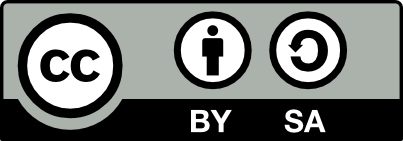
\includegraphics{figuras/cc-by-sa.png}
\end{center}

%%%%%%%%%%%%%%%%%%%%%%%%% Exceções da Licença CC-BY-SA %%%%%%%%%%%%%%%%%%%%%%%%%

A marca e o logotipo da UNICAMP são propriedade da Universidade Estadual de
Campinas. Maiores informações sobre encontram-se disponíveis em
\url{http://www.unicamp.br/unicamp/a-unicamp/logotipo/normas%20oficiais-para-uso-do-logotipo}.

\section{Sobre a licença dessa obra}
A licença Creative Commons Atribuição-CompartilhaIgual 3.0 Não Adaptada
utilizada nessa obra diz que:
\begin{enumerate}
  \item Você tem a liberdade de:
    \begin{itemize}
      \item Compartilhar — copiar, distribuir e transmitir a obra;
      \item Remixar — criar obras derivadas;
      \item fazer uso comercial da obra.
    \end{itemize}
  \item Sob as seguintes condições:
    \begin{itemize}
      \item Atribuição — Você deve creditar a obra da forma especificada pelo
        autor ou licenciante (mas não de maneira que sugira que estes concedem
        qualquer aval a você ou ao seu uso da obra).
      \item Compartilhamento pela mesma licença — Se você alterar, transformar
        ou criar em cima desta obra, você poderá distribuir a obra resultante
        apenas sob a mesma licença, ou sob uma licença similar à presente.
    \end{itemize}
\end{enumerate}

%
\backmatter
\end{lstlisting}


\section{Informações adicionais}
Perguntei para a Agência de Inovação da UNICAMP sobre quem detém os direitos
autorais das dissertações de mestrado e teses de doutorado e recebi a seguinte
resposta:

\begin{verbatim}
Date: Fri, 8 Mar 2013 08:41:22 -0300
From: Gabriel Gustavo Guion <gguion@inova.unicamp.br>
To: Raniere Silva <ra092767@ime.unicamp.br>
Cc: patentes@inova.unicamp.br
Subject: Re: Direito Autoral de Dissertações/Teses

Prezado Raniere,

Todas as obras, literárias, artísticas ou científicas são passiveis de
serem protegidas por Direito Autoral. Portanto, sua tese/dissertação é sim
registrável.
Para maiores informações acesse:
http://www.bn.br/portal/?nu_pagina=28

No caso da Unicamp, segundo nossa política de Propriedade Intelectual
instaurada pela deliberação *CONSU*-A-016/2010 de 30/11/2010, os direitos
de propriedade das criações literárias, artísticas e pedagógicas
pertencerão aos autores.

Estamos a disposição.

Atenciosamente.
Gabriel Guion
Gerente de Propriedade Intelectual

Agência de Inovação Inova Unicamp
(19) 3521-2549
www.inova.unicamp.br
\end{verbatim}

Deste modo, você como autor da sua dissertação de mestrado ou tese de
doutorado pode optar por utilizar uma licença copyleft, por exemplo CC-BY ou
CC-BY-SA, para a mesma.

É comum as informações de licenciamento de materiais impressos vir logo no
início do mesmo como é o caso na maioria dos livros (muitas vezes na mesma
página contendo a ficha catalográfica). Infelizmente como atualmente não existe
nenhuma normativa da UNICAMP especificando a posição da menção dos direitos
autorais das dissertações de mestrado e teses de doutorado acreditamos que o
melhor lugar para conter essa informação seja o último anexo\footnote{Isso
baseado no uso da licença GNU Free Documentation License (para maiores
informações visite \url{http://www.gnu.org/copyleft/fdl.html}}.
